\documentclass{article}
\usepackage[spanish]{babel}
\usepackage{amsmath, amsthm, amssymb}
\usepackage{graphicx}
\usepackage{url}
\usepackage[papersize={210mm,300mm},tmargin=15mm,bmargin=15mm]{geometry}
\begin{document}
\title{Proyecto de Programación 1er Semestre}
\author{Dylan Ramses Cabrera Morales\\ \\
\small{Grupo:C-122}}
\maketitle
Este proyecto consiste en un sistema de recuperacion de información que tiene como objetivo realizar una búsqueda
en un conjunto de archivos. La idea central de este es facilitar la búsqueda del usuario y hacerla
lo mas óptima posible. La interfaz gráfica ha sido programada en su mayoría con HTML y CSS, mientras
que el código de la búsqueda fue implementado en $C\sharp$.\\
Para ejecutar el proyecto debe leer Moogle.md\\ \\
Las clases utilizadas para la lógica del proyecto son:\\
\textbf{ProcesarDocumentos, Busqueda, Consulta, Moogle, SearchItem, SearchResult y Matriz}\\ \\
Al ejecutarse el proyecto inmediatamente se procede a llamar a la clase \textbf{\underline{ProcesarDocumentos}}.
 Dicha clase es la encargada de almacenar todos los archivos de texto que se encuentran ubicados en
 la carpeta Content en una Lista que contiene una Lista de las palabras de cada documento(Lista de Listas).\\
 Este proceso lo realiza el metodo \textbf{\underline{CargarDocumentos}} de la clase \textbf{\underline{ProcesarDocumentos}}.
 En este se ejecutan las siguientes funciones:
 \begin{enumerate}
    \item \underline{LeerTextos}: Devuelve una lista de documentos que contiene un listado de cada palabra que aparece en un documento. Para lograr esto, se invocan los metodos \textbf{ObtenerDocumentos} y \textbf{Tokenizar}.
    \begin{enumerate}
        \item \textbf{ObtenerDocumentos} devuelve las rutas de todos los documentos de la carpeta Content, mientras que \textbf{Tokenizar} se encarga de 
        evitar la aparición de signos de puntuación(esto lo realiza mediante la función \textbf{ModificarTexto}) y luego
        separa las palabras y las almacena en una lista de palabras
    \end{enumerate}
  \begin{figure}[h]
    \centering
    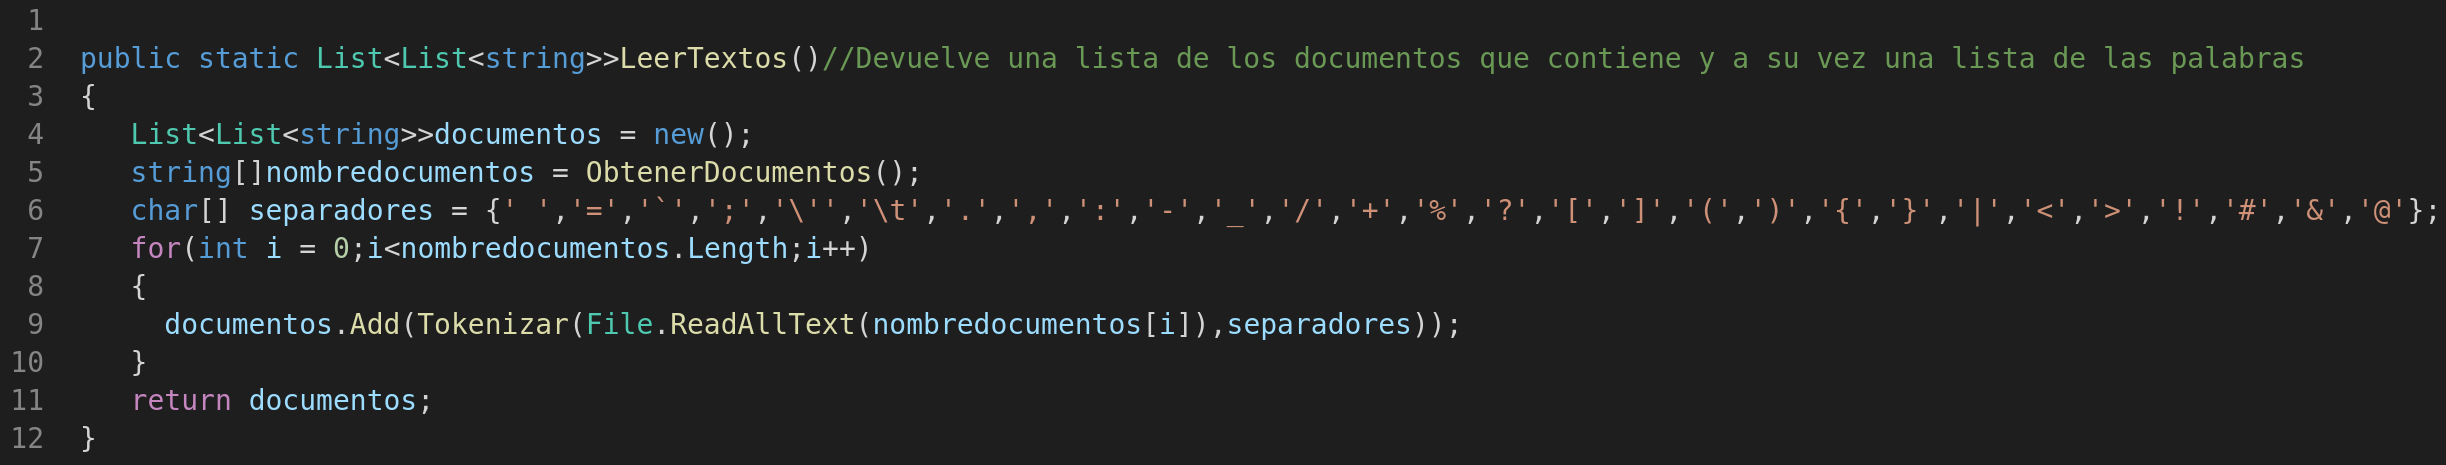
\includegraphics[width = 15cm]{fig 1.png}
    \caption{Método LeerTextos}
    \label{fig:1}
  \end{figure}
      \item \underline{CalcularTFIDF}: Su objetivo es calcular el TFIDF de todos los documentos(Para
      más información sobre este algoritmo:\url{https://es.ryte.com/wiki/TF*IDF}). Al finalizar su
      ejecución tendremos los valores del TF almacenados en una lista de diccionarios y el IDF en
      un diccionario independiente
      \item \underline{TFIDF}: Devuelve una lista de diccionarios con el valor del TFIDF de cada
      documento
  \begin{figure}[h]
    \centering
    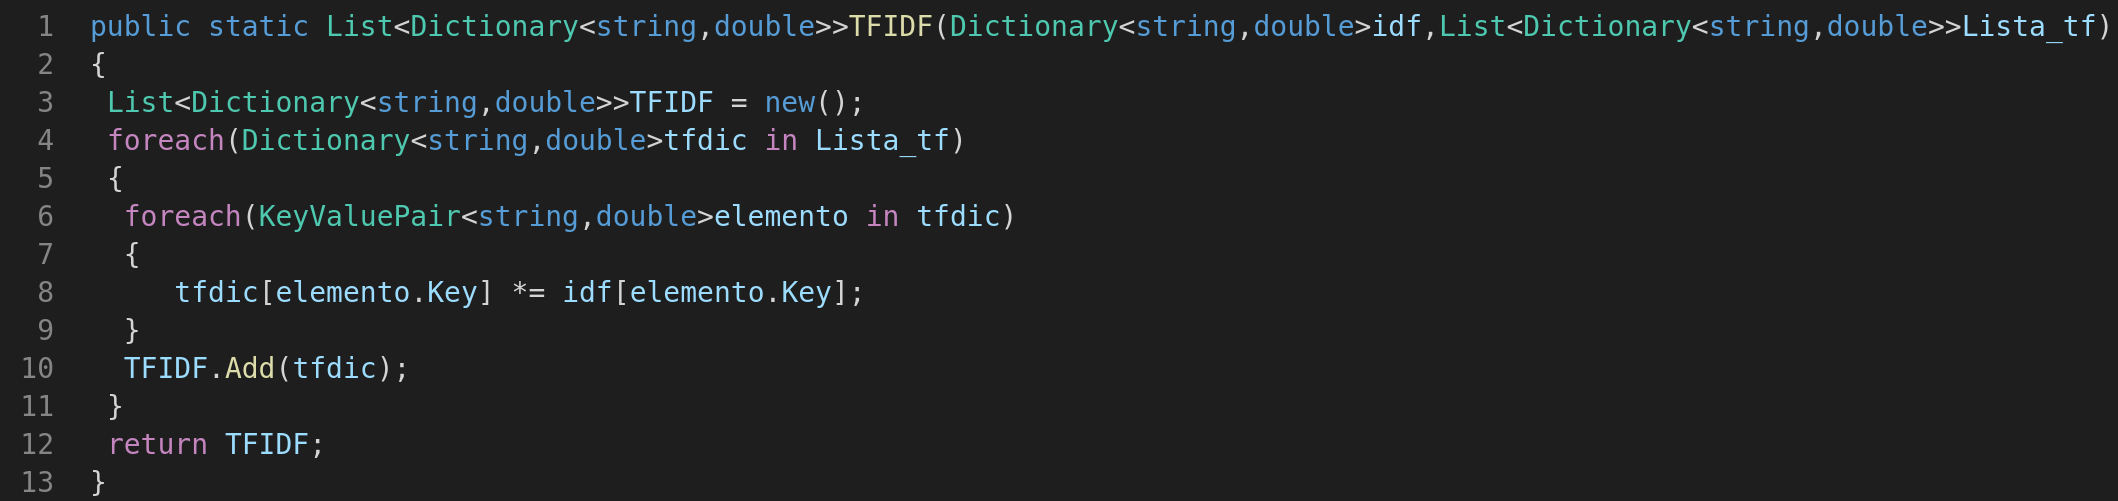
\includegraphics[width = 8cm]{fig 2.png}
    \caption{Metodo TFIDF}   
    \label{fig:2}
  \end{figure}
      \item \underline{Magnitud\_Documentos}: A partir del empleo del modelo vectorial, este método
      calcula la magnitud de un documento y lo devuelve como un array de valores de tipo double. 
      Este es un cálculo que solo se ejecuta una vez ya que no depende de la búsqueda(Para más 
      información:\url{https://www.sciencedirect.com/topics/computer-science/vector-space-models})  
  \begin{figure}[h]
    \centering
    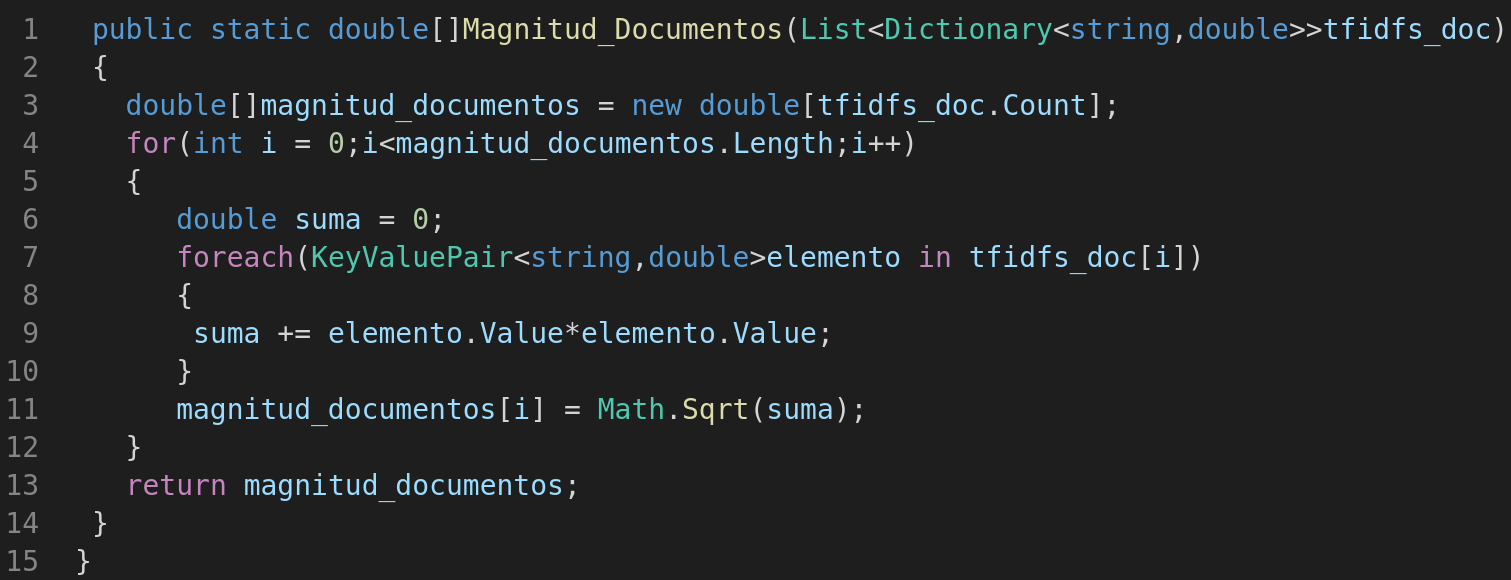
\includegraphics[width = 15cm]{fig 3.png}
    \caption{Método Magnitud\_Documentos}
    \label{fig:3}
  \end{figure}    
 \end{enumerate}
 Con esta información almacenada, se proceden a ejecutar las instrucciones de la clase \textbf{Moogle}.
 Una vez se introduce la búsqueda, la clase \textbf{Moogle} llama al método \textbf{Tokenizar} de 
 la clase \textbf{ProcesarDocumentos}, para separar las palabras de la query y almacenarlas en
 una lista de palabras. Luego se ejecutan una serie de funciones de la clase \textbf{Consulta}:
 \begin{enumerate}
  \item \underline{TFIDF\_Query}: Se encarga de calcular el TFIDF de la query
  \item \underline{Magnitud\_Query}: Calcula la magnitud de la query
   \item \underline{SimilitudCosenos}: Emplea el modelo vectorial para calcular la similitud de
   cosenos de los documentos y lo devuelve como un array de double
 \end{enumerate}
 En este punto ya tendremos los documentos más relevantes con respecto a la búsqueda, donde entra
 en juego la clase \textbf{Busqueda} para obtener un fragmento del documento que contiene parte de
 la búsqueda. Desde la clase principal \textbf{Moogle} se llaman los siguientes métodos de
 \textbf{Busqueda}:
 \begin{itemize}
  \item \underline{PosiciondelosDocumentosImportantes}: Es el método que devuelve la posición que
  ocupa en el array de similitud de cosenos los documentos más importantes. Si no se encuentra
  ningún documento similar retorna -1 
 \end{itemize} 
 A partir de aquí se divide en dos variantes: si se encuentran los resultados y si no se
 encuentran
 \begin{enumerate}
  \item Si son encontrados:
  \begin{enumerate}
    \item \underline{DocumentosImportantes}: Devuelve la ruta de los documentos más importantes
    ordenados 
    \begin{figure}[h]
      \centering
      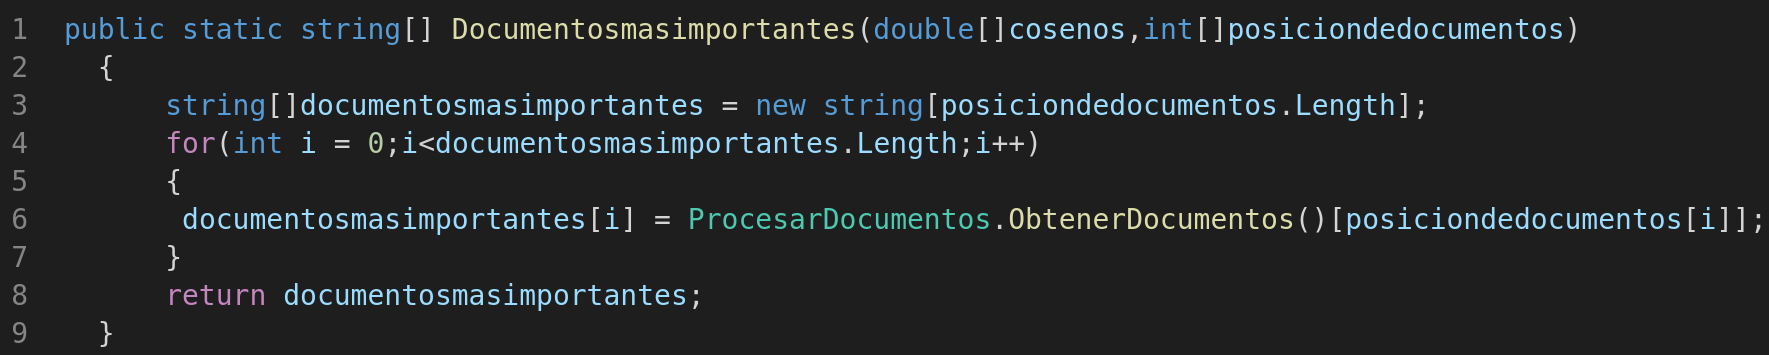
\includegraphics[width = 15cm]{fig 4.png}
      \caption{Metodo DocumentosImportantes}
      \label{fig:4}
    \end{figure}
    \item \underline{ObtenerSnippet}: Devuelve un fragmento del texto original que contenga parte
    de la query
  \end{enumerate}
  \item Si no son encontrados:
  \begin{enumerate}
    \item Se aplica un algoritmo de distancia entre palabras para encontrar aquellas que más se
    parecen a la query. Se llama al método \textbf{Sugerencia} de la clase \textbf{Consulta} que
    realiza esta función mediante el método \textbf{Similar}. Esto permite al usuario la opción
    de realizar una nueva búsqueda que si tendra resultados 
  \end{enumerate}
 \end{enumerate}
 La clase \textbf{Matriz} nunca se utliza. Fue implentada para la evaluacion de Álgebra
\end{document}